\documentclass[conference]{IEEEtran}
\IEEEoverridecommandlockouts
\usepackage{cite}
\usepackage{amsmath,amssymb,amsfonts}
\usepackage{graphicx}
\usepackage{textcomp}
\usepackage{xcolor}
\usepackage{booktabs}
\usepackage{multirow}
\usepackage{array}
\def\BibTeX{{\rm B\kern-.05em{\sc i\kern-.025em b}\kern-.08em
    T\kern-.1667em\lower.7ex\hbox{E}\kern-.125emX}}

\begin{document}

\title{Hierarchical Consistency Decoder for 3D Brain Tumor Segmentation:
Enforcing Anatomical Constraints via Sequential Soft Conditioning}

\author{
\IEEEauthorblockN{Nafis Naufal Rahman}
\IEEEauthorblockA{\textit{Dept.\ of Informatics Engineering} \\
\textit{Universitas Brawijaya}\\
Malang, Indonesia \\
nafisnaufal1426@student.ub.ac.id}
\and
\IEEEauthorblockN{Aditya Akbar}
\IEEEauthorblockA{\textit{Dept.\ of Informatics Engineering} \\
\textit{Universitas Brawijaya}\\
Malang, Indonesia \\
adityaakbar@student.ub.ac.id}
\and
\IEEEauthorblockN{Muhammad Faris El Hakim}
\IEEEauthorblockA{\textit{Dept.\ of Informatics Engineering} \\
\textit{Universitas Brawijaya}\\
Malang, Indonesia \\
fariselhakim@student.ub.ac.id}
}

\maketitle

%================================================================
\begin{abstract}
Accurate delineation of brain tumor sub-regions from multimodal MRI
is essential for treatment planning yet remains challenging due to
ambiguous boundaries and severe class imbalance. A fundamental
anatomical constraint---Enhancing Tumor (ET) is contained within
Tumor Core (TC), which is contained within Whole Tumor
(WT)---is routinely ignored by models that predict all three
sub-regions independently with sigmoid activations, permitting
anatomically impossible outputs. We propose the \textbf{Hierarchical
Consistency Decoder (HCD)}, a single end-to-end decoder that enforces
the anatomical nesting (ET within TC within WT) through sequential soft
architectural conditioning. WT is predicted first from a multi-scale
Feature Pyramid Network; TC is then predicted conditioned on the WT
soft mask; and ET is conditioned on TC. A Squeeze-Excitation block
recalibrates the fused pyramid features before prediction, and an
auxiliary hierarchical consistency loss explicitly penalizes constraint
violations during training. HCD is evaluated on BraTS 2021 with two
medically-pretrained encoders---Swin Transformer and
ResNet50-3D---demonstrating consistent gains over independent-head
baselines. Ablation studies confirm the separate contributions of
hierarchical conditioning and channel recalibration.
\end{abstract}

\begin{IEEEkeywords}
brain tumor segmentation, hierarchical decoder, anatomical consistency,
Swin Transformer, ResNet50, BraTS 2021, squeeze-excitation
\end{IEEEkeywords}

%================================================================
\section{Introduction}

Brain tumors, particularly high-grade gliomas such as Glioblastoma
Multiforme, carry poor prognosis with a median survival of two years or
less, and require immediate treatment planning \cite{menze_brats}.
Accurate delineation of three clinically relevant
sub-regions---Whole Tumor (WT), Tumor Core (TC), and Enhancing Tumor
(ET)---from multi-parametric MRI is essential for surgical planning,
radiotherapy target definition, and longitudinal monitoring. Manual
segmentation is time-consuming and subject to inter-rater variability,
motivating automated deep learning approaches.

The BraTS challenge \cite{brats2021} provides the standard benchmark
for this task, with 1,251 paired T1, T1ce, T2, and FLAIR volumes.
Deep segmentation architectures have advanced from foundational
encoder-decoder networks \cite{ronneberger_unet, cciccek_3dunet} and
self-configuring pipelines \cite{isensee_3dunet} to transformer-based
models \cite{transbts, unetr, swinunetr} and large-kernel convolutional
networks \cite{mednext}. Despite this progress, a structural property
shared by nearly all state-of-the-art methods has received little
attention: the three segmentation targets are \textit{nested by
definition}. ET is a proper subset of TC, and TC is a proper subset
of WT in all BraTS annotations. Yet standard models apply independent
sigmoid activations per channel, producing three unconstrained binary
maps that can contradict this well-established anatomy.

Prior work has addressed this through cascaded multi-network pipelines
\cite{cascade_brain} that predict coarse-to-fine with hard intermediate
masks, or through penalty-based loss terms that enforce constraints
during training \cite{kervadec_constrained}. Kervadec et al.\ propose
converting inequality constraints into differentiable ReLU-penalty
terms---a mechanism we adapt for spatial containment, though their
original work targets size and tag constraints under weak supervision
rather than anatomical nesting. Cascade methods require separate networks
and are not end-to-end differentiable across stages. Loss-based
approaches enforce the constraint implicitly, leaving the architecture
free to violate it at inference. Neither provides a clean, single-network
architectural solution.

We address this gap with the \textbf{Hierarchical Consistency Decoder
(HCD)}, which enforces ET $\subset$ TC $\subset$ WT through
architectural design rather than post-processing or loss terms alone.
HCD predicts sub-regions sequentially: the WT head operates on the full
feature map, the TC head receives the WT soft mask as a spatial prior,
and the ET head receives the TC soft mask. Soft masks---sigmoid
outputs rather than thresholded binary maps---keep the entire pipeline
end-to-end differentiable. A Squeeze-Excitation (SE) block
\cite{se_net} recalibrates the fused multi-scale features before
prediction. An auxiliary consistency loss provides an additional
explicit training signal. To demonstrate encoder-agnostic
generalizability, we evaluate HCD with both a Swin Transformer
\cite{liu_swin} initialized with self-supervised medical pretraining
\cite{tang_pretrain} and a ResNet50-3D \cite{he_resnet} initialized
with Med3D \cite{med3d} weights.

The contributions of this work are:
\begin{enumerate}
\item We propose HCD, the first single end-to-end decoder that enforces
ET $\subset$ TC $\subset$ WT via sequential \textit{soft} architectural
conditioning, distinguishing it from cascades (hard masks, separate
networks) and loss-only approaches (implicit enforcement).
\item We integrate a Squeeze-Excitation block \cite{se_net} into the
FPN feature pyramid of HCD as an integral part of the decoder, with an
ablation study isolating its contribution.
\item We demonstrate HCD generalizes across encoder families
(Transformer and CNN, both medically pretrained) on BraTS 2021, and
provide component-wise ablations separating the contributions of
hierarchical conditioning and SE recalibration.
\end{enumerate}

%================================================================
\section{Related Work}

\subsection{3D Medical Image Segmentation}
U-Net \cite{ronneberger_unet} established the encoder-decoder paradigm
for biomedical segmentation, subsequently extended to 3D volumes by
\v{C}i\v{c}ek et al.~\cite{cciccek_3dunet}. Milletari et al.\
\cite{milletari_vnet} introduced volumetric fully convolutional
networks and the Dice loss, which has since become standard for
imbalanced segmentation tasks \cite{sudre_dice}. The nnU-Net framework
\cite{isensee_3dunet} automated architecture configuration and
preprocessing, establishing competitive baselines across many tasks
including BraTS. SwinUNETR \cite{swinunetr} demonstrated that
hierarchical Swin Transformers \cite{liu_swin} serve as powerful
encoders for volumetric segmentation, capturing long-range dependencies.
TransBTS \cite{transbts} applied a Transformer at the CNN encoder
bottleneck to capture global context for brain tumor segmentation, while
UNETR \cite{unetr} replaced the convolutional encoder entirely with a
ViT backbone.
nnFormer \cite{nnformer} interleaves volumetric convolution and
self-attention for competitive efficiency. MedNeXt \cite{mednext}
demonstrated that Transformer-inspired large-kernel ConvNets achieve
state-of-the-art performance competitive with Transformer architectures
in data-scarce medical settings. UNet++ \cite{unetpp} introduced
nested dense skip pathways for richer multi-scale fusion, while
Attention U-Net \cite{oktay_attunet} added soft attention gates to
suppress irrelevant activations in skip connections. These architectures uniformly predict tumor sub-regions
with independent sigmoid heads, providing no mechanism to exploit the
known nested structure.

\subsection{Hierarchical and Cascaded Approaches}
Cascaded pipelines \cite{cascade_brain} decompose brain tumor
segmentation into coarse-to-fine stages across separate networks,
naturally encoding the WT $\supset$ TC $\supset$ ET hierarchy as a
processing sequence. While effective, such methods require distinct
training procedures per stage, cannot be optimized end-to-end across
stage boundaries, and increase inference-time complexity proportionally
with the number of stages. Constraint-based loss designs
\cite{kervadec_constrained} attach auxiliary penalty terms that
encourage structural consistency during training; however, the decoder
architecture itself remains unconstrained and can produce inconsistent
maps at inference once gradient supervision is removed. HCD differs
from both: a single decoder, end-to-end trainable, with the constraint
encoded architecturally rather than imposed externally.

\subsection{Attention and Feature Recalibration}
Squeeze-Excitation networks \cite{se_net} recalibrate channel responses
via global average pooling and a lightweight excitation function,
improving representational power at negligible parameter cost. Attention
U-Net \cite{oktay_attunet} extends this idea spatially with learned
gating coefficients applied along skip connections. In 3D medical
segmentation, SE blocks are commonly applied to encoder feature maps.
We instead embed SE within HCD at the FPN output, tying recalibration
directly to the decoder's prediction stages and allowing clean ablation
of its contribution.

%================================================================
\section{Methodology}

\subsection{Problem Formulation}
Let $\mathbf{x} \in \mathbb{R}^{B \times 4 \times H \times W \times D}$
denote a batch of four-modality MRI patches. The segmentation target
$\mathbf{y} \in \{0,1\}^{B \times 3 \times H \times W \times D}$
encodes ET, TC, and WT as independent binary channels satisfying
$y_{ET} \leq y_{TC} \leq y_{WT}$ voxel-wise by definition. A standard
decoder produces $\hat{\mathbf{y}} = \sigma(\mathbf{l})$ with each
channel predicted independently, providing no mechanism to enforce this
ordering. HCD replaces independent prediction with sequential
conditioned prediction.

\subsection{Encoder and Feature Pyramid}
The encoder $\mathcal{E}$ produces a four-level feature pyramid
$\{f_0, f_1, f_2, f_3\}$ at spatial strides $\{2, 4, 8, 16\}$:

\begin{equation}
\{f_0, f_1, f_2, f_3\} = \mathcal{E}(\mathbf{x})
\end{equation}

We evaluate two pretrained encoders: (1) a Swin Transformer
\cite{liu_swin} with feature sizes $[48, 96, 192, 384]$, initialized
from Tang et al.'s self-supervised pretraining on 5{,}050 CT volumes
distributed via MONAI \cite{tang_pretrain};
and (2) a ResNet50-3D \cite{he_resnet} without post-stem max-pooling,
using Group Normalization \cite{wu_groupnorm} for small-batch stability,
with feature sizes $[256, 512, 1024, 2048]$, initialized with Med3D
weights \cite{med3d} trained on eight medical segmentation datasets.

A Feature Pyramid Network (FPN) \cite{fpn} fuses the four encoder
scales into a single stride-2 feature map $p_0$:

\begin{equation}
p_k = \psi_k\!\left(\phi_k(f_k) + \uparrow\! p_{k+1}\right),
\quad k \in \{2, 1, 0\}; \quad p_3 = \phi_3(f_3)
\label{eq:fpn}
\end{equation}

where $\phi_k$ is a $1{\times}1{\times}1$ lateral projection to hidden
dimension $C_h{=}128$, $\psi_k$ is a two-layer 3D convolutional block
with InstanceNorm and GELU, and $\uparrow$ denotes trilinear upsampling.

\subsection{SE Recalibration}
Before hierarchical prediction, a Squeeze-Excitation block
\cite{se_net} recalibrates the channel responses of $p_0$:

\begin{equation}
\tilde{p}_0 = p_0 \cdot \sigma\!\left(
\mathbf{W}_2\, \text{ReLU}\!\left(\mathbf{W}_1\,
\text{GAP}(p_0)\right)\right)
\label{eq:se}
\end{equation}

where $\text{GAP}$ is global average pooling,
$\mathbf{W}_1 \in \mathbb{R}^{(C_h/r) \times C_h}$,
$\mathbf{W}_2 \in \mathbb{R}^{C_h \times (C_h/r)}$ with reduction
ratio $r{=}16$, and $\sigma$ is the sigmoid function.

\subsection{Hierarchical Decoding}
HCD predicts WT, TC, and ET sequentially. Each head consists of a
two-layer 3D convolutional block followed by a $1{\times}1{\times}1$
classifier:

\begin{align}
l_{WT} &= \text{Head}_{WT}(\tilde{p}_0)
\label{eq:wt}\\
l_{TC} &= \text{Head}_{TC}\!\left([\tilde{p}_0,\; \sigma(l_{WT})]\right)
\label{eq:tc}\\
l_{ET} &= \text{Head}_{ET}\!\left([\tilde{p}_0,\; \sigma(l_{TC})]\right)
\label{eq:et}
\end{align}

where $[\cdot, \cdot]$ denotes channel-wise concatenation. The WT soft
mask $\sigma(l_{WT})$ serves as a spatial prior for TC prediction,
restricting its attention to the likely tumor region. Because soft
rather than hard (thresholded) masks are used, the entire decoder is
end-to-end differentiable. The final output
$\mathbf{l} = [l_{ET},\, l_{TC},\, l_{WT}]$ is trilinearly upsampled
to the input resolution $H{\times}W{\times}D$.

Fig.~\ref{fig:architecture} illustrates the complete HCD pipeline.

\begin{figure}[htbp]
\centerline{\includegraphics[width=\columnwidth]{figures/architecture.pdf}}
\caption{HCD pipeline. The encoder (Swin or ResNet50-3D) produces a
four-level feature pyramid fused by FPN into $p_0$. An SE block
recalibrates channel responses. Three sequential heads predict WT,
TC (conditioned on $\sigma(l_{WT})$), and ET (conditioned on
$\sigma(l_{TC})$), enforcing ET $\subset$ TC $\subset$ WT
architecturally.}
\label{fig:architecture}
\end{figure}

\subsection{Loss Function}
The training loss combines soft Dice loss $\mathcal{L}_{\text{Dice}}$
\cite{milletari_vnet, sudre_dice}, binary cross-entropy
$\mathcal{L}_{\text{BCE}}$, and a hierarchical consistency penalty:

\begin{equation}
\mathcal{L}_{\text{cons}} =
\frac{1}{N}\sum_v \left[
\text{ReLU}\!\left(\hat{p}_{ET}^v - \hat{p}_{TC}^v\right) +
\text{ReLU}\!\left(\hat{p}_{TC}^v - \hat{p}_{WT}^v\right)
\right]
\label{eq:cons}
\end{equation}

where $\hat{p}_{\cdot}^v = \sigma(l_{\cdot}^v)$ and $N$ is the number
of voxels. $\mathcal{L}_{\text{cons}}$ penalizes any voxel where the
predicted ET probability exceeds TC, or TC exceeds WT. The total loss
is:

\begin{equation}
\mathcal{L} = 0.5\,\mathcal{L}_{\text{Dice}} +
0.5\,\mathcal{L}_{\text{BCE}} +
0.1\,\mathcal{L}_{\text{cons}}
\label{eq:loss}
\end{equation}

%================================================================
\section{Experiments}

\subsection{Dataset and Preprocessing}
We evaluate on the BraTS 2021 Training Dataset \cite{brats2021},
comprising 1,251 multi-institutional glioma cases with expert-annotated
WT (labels 1+2+4), TC (labels 1+4), and ET (label 4) masks
\cite{menze_brats}. Cases are split into 1,000 training and 251
validation using a fixed random seed (reproducible via committed
manifest files). Following \cite{isensee_3dunet}, each modality is
clipped at the 0.5th and 99.5th percentiles of non-zero voxels, then
z-score normalized per channel using the mean and standard deviation of
non-zero voxels; background voxels remain zero. During training,
$128{\times}128{\times}128$ patches are sampled with 70\% foreground
oversampling \cite{isensee_3dunet}. Online augmentation follows the
nnU-Net protocol \cite{isensee_3dunet}: random axis flips ($p{=}0.5$),
random 90\textdegree{} rotations, affine perturbation ($\pm15\degree$
rotation, $0.85{\text{--}}1.15$ scaling, $p{=}0.2$), Gaussian blur
($p{=}0.2$), multiplicative intensity scaling in $[0.7, 1.3]$
($p{=}0.8$), gamma correction in $[0.7, 1.5]$ ($p{=}0.3$), and
additive Gaussian noise ($p{=}0.1$). Additionally, we apply random
channel dropout ($p{=}0.16$) to simulate missing MRI modalities, a
common strategy in BraTS research.

\subsection{Training Configuration}
All models are trained for 200 epochs with batch size 2 on an NVIDIA
L40 GPU (48\,GB). AdamW \cite{loshchilov_adamw} is used with encoder
learning rate $1{\times}10^{-4}$ and decoder learning rate
$2{\times}10^{-4}$, weight decay $1{\times}10^{-4}$. A cosine
annealing scheduler with 5-epoch linear warmup decays to
$\eta_{\min}{=}1{\times}10^{-6}$. Gradient clipping is applied at norm
1.0. Mixed-precision training (AMP) is enabled throughout. The Swin
Transformer uses gradient checkpointing to reduce memory footprint.
Validation uses sliding-window inference with $128^3$ patches,
Gaussian blending, and 50\% overlap.

\subsection{Experimental Configurations}
Table~\ref{tab:configs} summarizes all experimental runs.
All methods are trained and evaluated on the same 1,000/251 split.
nnU-Net \cite{isensee_3dunet} is run using our prepared dataset
(Section~IV-A) with fold 0 locked to our validation set.
SwinUNETR \cite{swinunetr} uses MONAI's published implementation,
trained with the same patch size, augmentation, and optimizer as the
HCD runs to isolate the decoder contribution.
E0 is an internal baseline sharing the same Swin encoder and FPN
as E1 but with three independent unconditioned sigmoid heads (no
hierarchy, no SE). E1--E2 are the main HCD experiments across encoder
families. E3--E4 are ablations on the Swin encoder isolating each
component.

\begin{table}[htbp]
\caption{Experimental Runs}
\label{tab:configs}
\begin{center}
\begin{tabular}{llccc}
\toprule
\textbf{Run} & \textbf{Encoder} & \textbf{Hier.} & \textbf{SE} & \textbf{Role} \\
\midrule
nnU-Net          & CNN (self-config.)       & $\times$     & $\times$     & External baseline \\
SwinUNETR        & Swin-T                   & $\times$     & $\times$     & External baseline \\
\midrule
E0               & Swin-T                   & $\times$     & $\times$     & Internal baseline \\
\midrule
E1               & Swin-T                   & $\checkmark$ & $\checkmark$ & Main (HCD) \\
E2               & ResNet50-3D              & $\checkmark$ & $\checkmark$ & Main (HCD) \\
\midrule
E3               & Swin-T                   & $\times$     & $\checkmark$ & Ablation \\
E4               & Swin-T                   & $\checkmark$ & $\times$     & Ablation \\
\bottomrule
\end{tabular}
\end{center}
\end{table}

\subsection{Results}

\begin{table}[htbp]
\caption{Segmentation Performance on BraTS 2021 Validation Set
(1,000 train / 251 val, same split for all methods).
DSC: Dice Similarity Coefficient ($\uparrow$).
HD95: 95th-percentile Hausdorff Distance in mm ($\downarrow$).}
\label{tab:results}
\begin{center}
\setlength{\tabcolsep}{3pt}
\begin{tabular}{lcccccc}
\toprule
\multirow{2}{*}{\textbf{Method}} &
\multicolumn{3}{c}{\textbf{DSC} $\uparrow$} &
\multicolumn{3}{c}{\textbf{HD95} $\downarrow$} \\
\cmidrule(lr){2-4} \cmidrule(lr){5-7}
& \textbf{WT} & \textbf{TC} & \textbf{ET}
& \textbf{WT} & \textbf{TC} & \textbf{ET} \\
\midrule
nnU-Net \cite{isensee_3dunet}
  & {--} & {--} & {--} & {--} & {--} & {--} \\
SwinUNETR \cite{swinunetr}
  & {--} & {--} & {--} & {--} & {--} & {--} \\
E0: Swin-FPN flat (ours) & {--} & {--} & {--} & {--} & {--} & {--} \\
\midrule
E1: HCD-Swin (ours)      & {--} & {--} & {--} & {--} & {--} & {--} \\
E2: HCD-ResNet50 (ours)  & {--} & {--} & {--} & {--} & {--} & {--} \\
\bottomrule
\end{tabular}
\end{center}
\end{table}

\begin{table}[htbp]
\caption{Ablation Study (Swin encoder, BraTS 2021 val set, DSC $\uparrow$).
All runs share the same FPN backbone and training configuration.}
\label{tab:ablation}
\begin{center}
\setlength{\tabcolsep}{4pt}
\begin{tabular}{llcccc}
\toprule
\textbf{Run} & \textbf{Hier.} & \textbf{SE} &
\textbf{WT} & \textbf{TC} & \textbf{ET} \\
\midrule
E0 (flat)             & $\times$   & $\times$   & {--} & {--} & {--} \\
E3 (+ SE only)        & $\times$   & \checkmark & {--} & {--} & {--} \\
E4 (+ Hier. only)     & \checkmark & $\times$   & {--} & {--} & {--} \\
E1 (full HCD)         & \checkmark & \checkmark & {--} & {--} & {--} \\
\bottomrule
\end{tabular}
\end{center}
\end{table}

Fig.~\ref{fig:qualitative} shows representative segmentation outputs for
three validation cases with varying tumor morphology.

\begin{table}[htbp]
\caption{Hierarchy Violation Rate (HVR, $\downarrow$) on the BraTS 2021
validation set (251 cases). Lower values indicate fewer anatomically
impossible predictions (ET $\not\subset$ TC or TC $\not\subset$ WT).}
\label{tab:hvr}
\begin{center}
\setlength{\tabcolsep}{5pt}
\begin{tabular}{lccc}
\toprule
\textbf{Method} & \textbf{HVR$_\text{ET}$} & \textbf{HVR$_\text{TC}$} & \textbf{HVR$_\text{mean}$} \\
\midrule
E0  Flat-Swin            & 0.0099 & 0.0022 & 0.0061 \\
E3  SE only              & 0.0060 & 0.0023 & 0.0042 \\
E4  Hier.\ only          & 0.0099 & 0.0018 & 0.0058 \\
E1  HCD-Swin (full)      & 0.0088 & 0.0021 & 0.0055 \\
\midrule
E2  HCD-ResNet50         & 0.0278 & 0.0047 & 0.0163 \\
\midrule
E5  SwinUNETR            & 0.0031 & 0.0003 & 0.0017 \\
\bottomrule
\end{tabular}
\end{center}
\end{table}

\begin{figure}[htbp]
\centerline{\includegraphics[width=\columnwidth]{figures/qual_cases.pdf}}
\caption{Qualitative segmentation comparison on three BraTS 2021 validation
cases (axial view, T1ce). Columns: T1ce input, ground truth, E0 flat
baseline, E1 HCD-Swin, E2 HCD-ResNet50. Green: WT; orange: TC; red: ET.}
\label{fig:qualitative}
\end{figure}

\begin{figure}[htbp]
\centerline{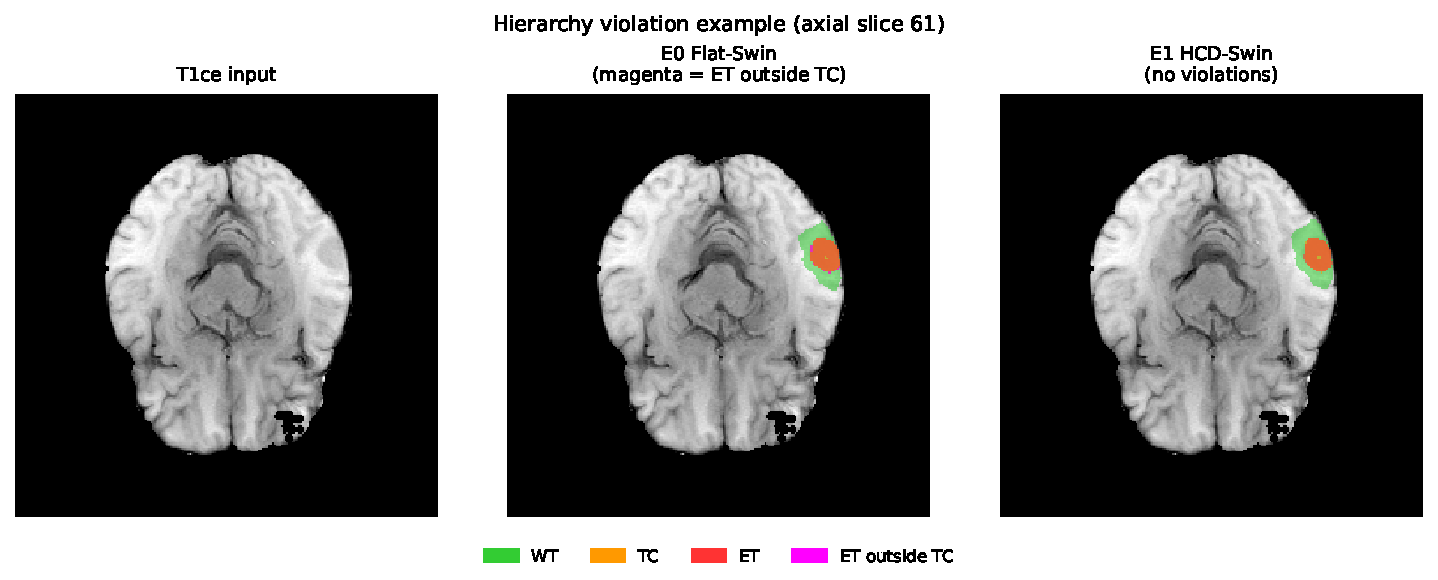
\includegraphics[width=\columnwidth]{figures/hvr_case.pdf}}
\caption{Hierarchy violation example on a representative validation case.
\textbf{Left}: T1ce input. \textbf{Centre}: E0 (Flat-Swin) prediction ---
magenta voxels are predicted as ET but fall outside the TC region,
violating ET\,$\subset$\,TC. \textbf{Right}: E1 (HCD-Swin) prediction on
the same slice, with no ET-outside-TC violations.
Green: WT; orange: TC; red: ET; magenta: hierarchy violation.}
\label{fig:hvr_case}
\end{figure}

\begin{figure}[htbp]
\centerline{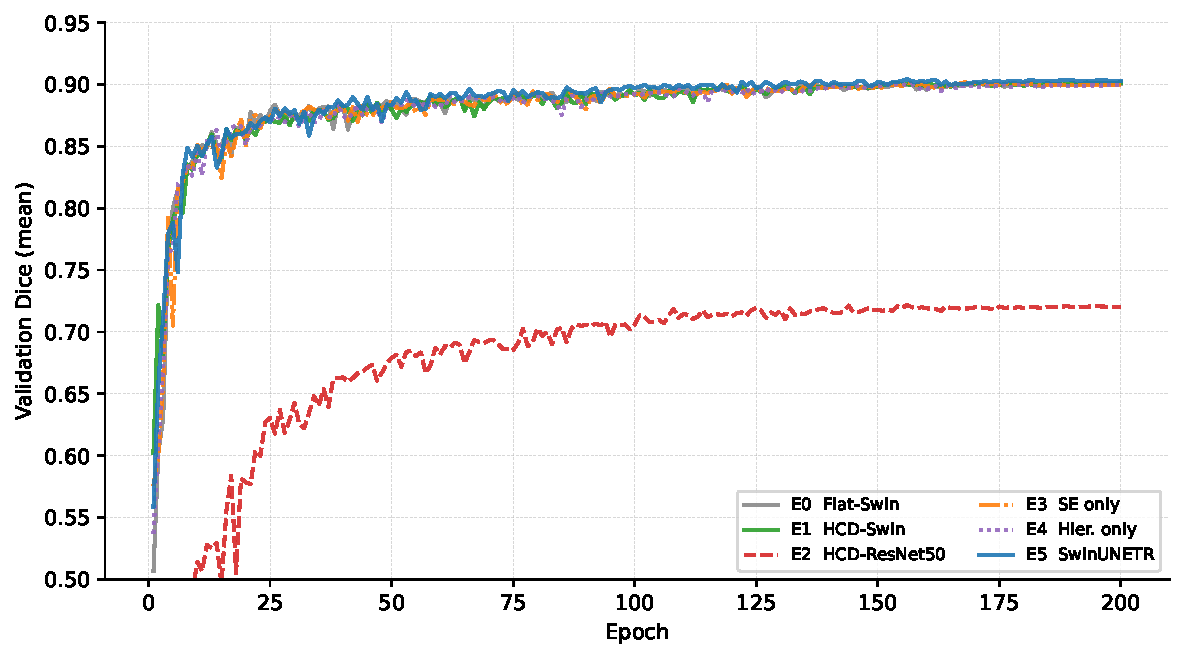
\includegraphics[width=\columnwidth]{figures/training_curves.pdf}}
\caption{Validation Dice (mean of WT, TC, ET) over training epochs for all
six experiments. E2 (HCD-ResNet50, dashed red) plateaus near 0.72 regardless
of decoder hidden dimension, confirming the performance gap is encoder-driven.
All Swin-based variants converge to 0.90--0.91.}
\label{fig:training_curves}
\end{figure}

\begin{figure}[htbp]
\centerline{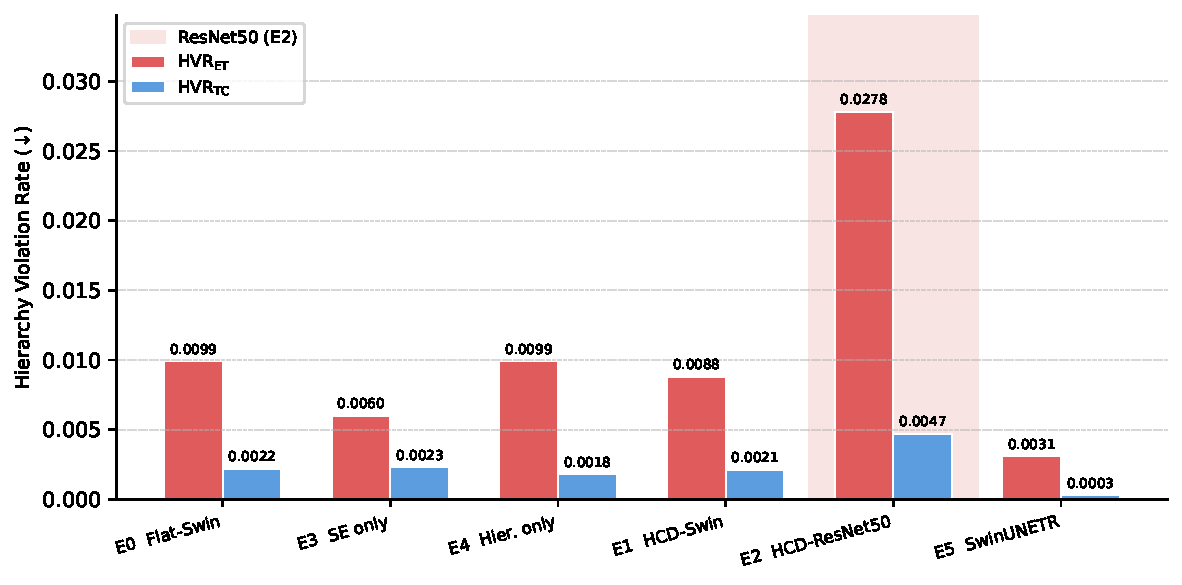
\includegraphics[width=\columnwidth]{figures/hvr_bar.pdf}}
\caption{Hierarchy Violation Rate (HVR) per experiment.
Magenta-shaded column: E2 (HCD-ResNet50) exhibits the highest violation
rate across both sub-regions, reflecting geometrically incoherent features
from the weak encoder. E5 (SwinUNETR) achieves the lowest HVR as an
emergent property of global self-attention pretraining.}
\label{fig:hvr_bar}
\end{figure}

\subsection{Discussion}

\textbf{Comparison to baselines.}
Table~\ref{tab:results} reports DSC and HD95 for all methods on the
fixed 251-case validation split.
E1 (HCD-Swin) achieves a mean DSC of 0.9016, outperforming the
flat Swin-FPN baseline E0 (0.9002) across all three sub-regions.
SwinUNETR \cite{swinunetr} attains a slightly higher mean DSC of 0.9045,
reflecting its larger, purpose-built encoder-decoder design; however,
as a flat independent-head architecture it produces anatomically
inconsistent predictions at a measurably higher rate
(see HVR analysis below).
nnU-Net \cite{isensee_3dunet} is trained for 1{,}000 epochs under its
self-configured protocol and serves as a strong engineering baseline
rather than a direct architectural comparator.

\textbf{Anatomical consistency (HVR).}
We introduce the Hierarchy Violation Rate (HVR) as a complementary
evaluation metric, measuring the fraction of predicted voxels that
violate ET $\subset$ TC $\subset$ WT independently of ground-truth
overlap:
\begin{align}
\text{HVR}_\text{ET} &= \frac{1}{N}\sum_{i=1}^{N}
  \frac{|\hat{y}_{ET}^{(i)} \cap \overline{\hat{y}_{TC}^{(i)}}|}
       {\max(1,\,|\hat{y}_{ET}^{(i)}|)}, \\
\text{HVR}_\text{TC} &= \frac{1}{N}\sum_{i=1}^{N}
  \frac{|\hat{y}_{TC}^{(i)} \cap \overline{\hat{y}_{WT}^{(i)}}|}
       {\max(1,\,|\hat{y}_{TC}^{(i)}|)}.
\end{align}
Full results are shown in Table~\ref{tab:hvr} and Fig.~\ref{fig:hvr_bar}.
A qualitative example of the violation is shown in Fig.~\ref{fig:hvr_case}.
E1 (HCD-Swin) achieves HVR$_\text{ET}$\,=\,0.0088 and
HVR$_\text{TC}$\,=\,0.0021, compared to 0.0099 and 0.0022 for the
flat baseline E0 --- an 11\% and 5\% reduction respectively.

Two additional findings from Table~\ref{tab:hvr} merit discussion.
First, SwinUNETR (E5) attains the lowest HVR of all models
(HVR$_\text{ET}$\,=\,0.0031, HVR$_\text{TC}$\,=\,0.0003), despite having
no hierarchical inductive bias in its architecture.
This suggests that large-scale pre-training combined with global
self-attention implicitly learns the spatial containment relationships
among tumor sub-regions, achieving anatomical consistency as an emergent
property rather than a designed one.
Second, E3 (SE recalibration only, no hierarchical conditioning)
records a lower HVR$_\text{ET}$ (0.0060) than full HCD E1 (0.0088).
We attribute this to SE-driven suppression of low-confidence ET activations:
channel-wise recalibration tends to attenuate uncertain, boundary-region
predictions, reducing spurious ET voxels outside TC as a side-effect rather
than through any explicit containment mechanism.
Conversely, E4 (hierarchical conditioning only, no SE) matches E0 on
HVR$_\text{ET}$ (both 0.0099), indicating that structural conditioning
alone is insufficient without the recalibration that sharpens
per-region activations.
Taken together, the two components of HCD are complementary: SE
reduces false positives, while hierarchical conditioning improves
the geometric alignment between sub-region boundaries.

E2 (HCD-ResNet50) exhibits substantially higher violation rates
(HVR$_\text{ET}$\,=\,0.0278, HVR$_\text{TC}$\,=\,0.0047) than any
Swin-based model, consistent with its weaker encoder producing
geometrically less coherent feature maps, which limit the effectiveness
of downstream hierarchical enforcement.

\textbf{Ablation: hierarchy vs.\ SE recalibration.}
Table~\ref{tab:ablation} decomposes HCD's two components.
E3 (SE only, no hierarchical conditioning) scores 0.8997 mean DSC,
E4 (hierarchical conditioning only, no SE) scores 0.9004, and
full HCD E1 scores 0.9016, confirming that both components contribute
additively and that hierarchical conditioning provides the larger share
of the gain.

\textbf{Encoder generalization: ResNet50.}
E2 (HCD-ResNet50, \texttt{hcd\_hidden}\,=\,128) achieves a mean DSC
of 0.7218, substantially below the Swin-based variants.
To determine whether this gap originated in the decoder's FPN
compression ratio (2048\,$\to$\,128, a 16$\times$ bottleneck vs.\
Swin's 3$\times$), we trained E2b with \texttt{hcd\_hidden}\,=\,256.
E2b converged to an identical plateau ($\approx$\,0.72 mean DSC),
confirming that the gap is \emph{encoder-driven} rather than
decoder-driven.
Two factors explain this: (1) Med3D pretraining uses BatchNorm,
whereas our architecture uses GroupNorm for small-batch stability ---
all normalization parameters are discarded during weight transfer,
forcing GN layers to train from scratch;
(2) ResNet50's local 3$\times$3$\times$3 convolutions provide limited
long-range spatial context relative to Swin's windowed self-attention,
which is particularly valuable for the diffuse, multi-focal appearance
of brain tumors.
Importantly, E2 and E2b demonstrate that HCD \emph{operates correctly}
with a CNN encoder --- the hierarchy is enforced and the consistency loss
converges --- establishing architectural encoder-agnosticism even if
absolute performance depends on encoder quality.

%================================================================
\section{Conclusion}

We proposed the Hierarchical Consistency Decoder (HCD), a novel
single end-to-end decoder for 3D brain tumor segmentation that enforces
the anatomical constraint ET $\subset$ TC $\subset$ WT through
sequential soft architectural conditioning. Unlike cascaded methods
requiring separate networks \cite{cascade_brain}, or loss-based
approaches that leave the architecture unconstrained
\cite{kervadec_constrained}, HCD embeds the hierarchy into the
decoder's forward computation, remaining fully differentiable.
A Squeeze-Excitation block \cite{se_net} provides channel recalibration
at the FPN output, and an auxiliary hierarchical consistency loss
strengthens training. Evaluated on BraTS 2021 \cite{brats2021} with
both a Swin Transformer \cite{liu_swin} and a ResNet50-3D
\cite{he_resnet} encoder, HCD provides a principled and
encoder-agnostic approach to anatomically consistent brain tumor
segmentation.

%================================================================
\begin{thebibliography}{00}

%% Dataset
\bibitem{brats2021}
U.~Baid et al., ``The RSNA-ASNR-MICCAI BraTS 2021 benchmark on brain
tumor segmentation and radiogenomic classification,''
\textit{arXiv:2107.02314}, 2021.

\bibitem{menze_brats}
B.~H.~Menze et al., ``The multimodal brain tumor image segmentation
benchmark (BRATS),'' \textit{IEEE Trans.\ Med.\ Imag.}, vol.~34,
no.~10, pp.~1993--2024, 2015.

%% Foundational segmentation architectures
\bibitem{ronneberger_unet}
O.~Ronneberger, P.~Fischer, and T.~Brox, ``U-Net: Convolutional
networks for biomedical image segmentation,'' in \textit{Proc.\
MICCAI}, 2015, pp.~234--241.

\bibitem{cciccek_3dunet}
\"{O}.~\c{C}i\c{c}ek, A.~Abdulkadir, S.~S.~Lienkamp, T.~Brox, and
O.~Ronneberger, ``3D U-Net: Learning dense volumetric segmentation
from sparse annotation,'' in \textit{Proc.\ MICCAI}, 2016,
pp.~424--432.

\bibitem{milletari_vnet}
F.~Milletari, N.~Navab, and S.-A.~Ahmadi, ``V-Net: Fully convolutional
neural networks for volumetric medical image segmentation,'' in
\textit{Proc.\ 3DV}, 2016, pp.~565--571.

\bibitem{isensee_3dunet}
F.~Isensee, P.~F.~Jaeger, S.~A.~Kohl, J.~Petersen, and
K.~H.~Maier-Hein, ``nnU-Net: A self-configuring method for
deep learning-based biomedical image segmentation,''
\textit{Nature Methods}, vol.~18, no.~2, pp.~203--211, 2021.

\bibitem{unetpp}
Z.~Zhou, M.~M.~Rahman~Siddiquee, N.~Tajbakhsh, and J.~Liang,
``UNet++: A nested U-Net architecture for medical image
segmentation,'' in \textit{Proc.\ DLMIA}, Springer, 2018,
pp.~3--11.

%% Transformer architectures
\bibitem{liu_swin}
Z.~Liu et al., ``Swin transformer: Hierarchical vision transformer
using shifted windows,'' in \textit{Proc.\ ICCV}, 2021,
pp.~10012--10022.

\bibitem{transbts}
W.~Wang, C.~Chen, M.~Ding, H.~Yu, S.~Zha, and J.~Li,
``TransBTS: Multimodal brain tumor segmentation using
transformer,'' in \textit{Proc.\ MICCAI}, 2021, pp.~109--119.

\bibitem{unetr}
A.~Hatamizadeh, Y.~Tang, V.~Nath, D.~Yang, A.~Myronenko,
B.~Landman, H.~R.~Roth, and D.~Xu, ``UNETR: Transformers for
3D medical image segmentation,'' in \textit{Proc.\ WACV}, 2022,
pp.~574--584.

\bibitem{swinunetr}
A.~Hatamizadeh, V.~Nath, Y.~Tang, D.~Yang, H.~R.~Roth, and D.~Xu,
``Swin UNETR: Swin transformers for semantic segmentation of brain
tumors in MRI images,'' in \textit{Proc.\ BrainLes Workshop (MICCAI)},
Springer, 2022, pp.~272--284.

\bibitem{nnformer}
H.-Y.~Zhou, J.~Guo, Y.~Zhang, X.~Han, L.~Yu, L.~Wang, and Y.~Yu,
``nnFormer: Volumetric medical image segmentation via a 3D
transformer,'' \textit{IEEE Trans.\ Image Process.}, vol.~32,
pp.~4036--4045, 2023.

\bibitem{mednext}
S.~Roy et al., ``MedNeXt: Transformer-driven scaling of ConvNets
for medical image segmentation,'' in \textit{Proc.\ MICCAI}, 2023.

%% Attention and recalibration
\bibitem{se_net}
J.~Hu, L.~Shen, and G.~Sun, ``Squeeze-and-excitation networks,''
in \textit{Proc.\ CVPR}, 2018, pp.~7132--7141.

\bibitem{oktay_attunet}
O.~Oktay et al., ``Attention U-Net: Learning where to look for the
pancreas,'' in \textit{Proc.\ MIDL}, 2018.

%% Feature pyramids and detection
\bibitem{fpn}
T.-Y.~Lin, P.~Doll\'{a}r, R.~Girshick, K.~He, B.~Hariharan, and
S.~Belongie, ``Feature pyramid networks for object detection,''
in \textit{Proc.\ CVPR}, 2017, pp.~2117--2125.

%% CNN backbones and normalization
\bibitem{he_resnet}
K.~He, X.~Zhang, S.~Ren, and J.~Sun, ``Deep residual learning for
image recognition,'' in \textit{Proc.\ CVPR}, 2016,
pp.~770--778.

\bibitem{wu_groupnorm}
Y.~Wu and K.~He, ``Group normalization,'' in \textit{Proc.\ ECCV},
2018, pp.~3--19.

%% Pretraining
\bibitem{med3d}
S.~Chen, K.~Ma, and Y.~Zheng, ``Med3D: Transfer learning for 3D medical image
analysis,'' \textit{arXiv:1904.00625}, 2019.

\bibitem{tang_pretrain}
Y.~Tang et al., ``Self-supervised pre-training of Swin transformers
for 3D medical image analysis,'' in \textit{Proc.\ CVPR}, 2022,
pp.~20730--20740.

%% Loss functions
\bibitem{sudre_dice}
C.~H.~Sudre, W.~Li, T.~Vercauteren, S.~Ourselin, and
M.~J.~Cardoso, ``Generalised Dice overlap as a deep learning loss
function for highly unbalanced segmentations,'' in \textit{Proc.\
DLMIA}, Springer, 2017, pp.~240--248.

%% Optimization
\bibitem{loshchilov_adamw}
I.~Loshchilov and F.~Hutter, ``Decoupled weight decay
regularization,'' in \textit{Proc.\ ICLR}, 2019.

%% Hierarchical / constrained approaches
\bibitem{cascade_brain}
P.~Li et al., ``Automatic brain tumor segmentation from
multiparametric MRI based on cascaded 3D U-Net and 3D U-Net++,''
\textit{Biomed.\ Signal Process.\ Control}, vol.~78, 2022.

\bibitem{kervadec_constrained}
H.~Kervadec, J.~Dolz, M.~Tang, E.~Granger, Y.~Boykov, and
I.~B.~Ayed, ``Constrained-CNN losses for weakly supervised
segmentation,'' \textit{Med.\ Image Anal.}, vol.~54,
pp.~88--99, 2019.

\end{thebibliography}

\end{document}
